%%%%%%%%%%%%%%%%%%%%%%%%%%%%%%%%%%%%%%%%%
% Class Notes Template
% LaTeX Template
% By: Ryan Grove
%%%%%%%%%%%%%%%%%%%%%%%%%%%%%%%%%%%%%%%%%

%----------------------------------------------------------------------------------------
%	PACKAGES AND OTHER DOCUMENT CONFIGURATIONS
%----------------------------------------------------------------------------------------

\documentclass[paper=a4, fontsize=11pt]{scrartcl} % A4 paper and 11pt font size

\usepackage[T1]{fontenc} % Use 8-bit encoding that has 256 glyphs
\usepackage{fourier} % Use the Adobe Utopia font for the document - comment this line to return to the LaTeX default
\usepackage[english]{babel} % English language/hyphenation
\usepackage{amsmath,amsfonts,amsthm} % Math packages

\usepackage{lipsum} % Used for inserting dummy 'Lorem ipsum' text into the template

\usepackage{sectsty} % Allows customizing section commands
\allsectionsfont{\centering \normalfont\scshape} % Make all sections centered, the default font and small caps

\usepackage{fancyhdr} % Custom headers and footers
\pagestyle{fancyplain} % Makes all pages in the document conform to the custom headers and footers
\fancyhead{} % No page header - if you want one, create it in the same way as the footers below
\fancyfoot[L]{} % Empty left footer
\fancyfoot[C]{} % Empty center footer
%\fancyfoot[R]{\thepage} % Page numbering for right footer
\renewcommand{\headrulewidth}{0pt} % Remove header underlines
\renewcommand{\footrulewidth}{0pt} % Remove footer underlines
\setlength{\headheight}{13.6pt} % Customize the height of the header

\numberwithin{equation}{section} % Number equations within sections (i.e. 1.1, 1.2, 2.1, 2.2 instead of 1, 2, 3, 4)
\numberwithin{figure}{section} % Number figures within sections (i.e. 1.1, 1.2, 2.1, 2.2 instead of 1, 2, 3, 4)
\numberwithin{table}{section} % Number tables within sections (i.e. 1.1, 1.2, 2.1, 2.2 instead of 1, 2, 3, 4)

\setlength\parindent{0pt} % Removes all indentation from paragraphs - comment this line for an assignment with lots of text

\usepackage{lastpage}
\usepackage{fancyhdr}
\cfoot{\thepage\ of \pageref{LastPage}}

\def\v{\hbox{$\mathbf v$}}
\def\w{\hbox{$\mathbf w$}}
\def\u{\hbox{$\mathbf u$}}
\def\x{\hbox{$\textbf{x}$}}
\def\z{\hbox{$\mathbf z$}}
\def\a{\hbox{$\mathbf a$}}
\def\b{\hbox{$\mathbf b$}}
\def\L{\hbox{$\mathcal L$}}
\def\C{\hbox{$\mathbb C$}}
\def\B{\hbox{$\mathcal B$}}
\def\R{\hbox{$\mathbb R$}}
\def\X{\hbox{$\underline X$}}
\def\Q{\hbox{$\mathbb Q$}}
\def\R{\hbox{$\mathbb R$}}
\def\N{\hbox{$\mathbb N$}}
\def\C{\hbox{$\mathbb C$}}
\def\0{\hbox{$\mathbf 0$}}
\def\Y{\hbox{$\underline Y$}}
\def\a{\hbox{$\mathbf a$}}
\def\u{\hbox{$\mathbf u$}}
\def\w{\hbox{$\mathbf w$}}
\def\y{\hbox{$\mathbf y$}}
\def\X{\hbox{$\underline X$}}
\def\dd{\hbox{$\partial $}}
\def\B{\hbox{$\mathcal B$}}
\def\F{\hbox{$\mathcal F$}}
\def\L{\hbox{$\mathcal L$}}
\def\M{\hbox{$\mathcal M$}}
\def\D{\hbox{$\mathscr {D}$}}
\def\RR{\hbox{$\mathscr{R}$}}
\def\I{\hbox{$\mathcal I$}}

\usepackage{amssymb}
%\theoremstyle{plain}
\usepackage[margin = .75in]{geometry}
\newtheorem{claim}{Claim}
\newtheorem{theorem}{Theorem}[section]
\newtheorem{lemma}[theorem]{Lemma}
\newtheorem{proposition}[theorem]{Proposition}
\newtheorem{corollary}[theorem]{Corollary}
\newtheorem{problem}[theorem]{Problem}
%\theoremstyle{definition}
\newtheorem{definition}[theorem]{Definition}
%\theoremstyle{remark}
\newtheorem{remark}[theorem]{Remark}
\newtheorem{remarks}[theorem]{Remarks}
\newtheorem{example}[theorem]{Example}
\newcommand{\ds}{\displaystyle}
\newcommand{\ZZ}{\mathbb{Z}}
\newcommand{\QQ}{\mathbb{Q}}
\newcommand{\e}{\varepsilon}
\newcommand{\bbf}{\textbf}
\newcommand{\p}{\parallel}
\usepackage{color}
\newcommand{\field}[1]{\mathbb{#1}}
\usepackage{amsmath}
\usepackage{amsthm}
\usepackage{amssymb}
\usepackage{mathrsfs}
\usepackage{cancel}
\usepackage{upgreek}
\usepackage{graphicx}
\usepackage{multirow}
\usepackage{setspace}
\usepackage{url}
\usepackage{subfigure}
\usepackage{enumerate}
\usepackage{cases}
\usepackage{mathrsfs}
\usepackage{rotating}

%----------------------------------------------------------------------------------------
%	TITLE SECTION
%----------------------------------------------------------------------------------------

\newcommand{\horrule}[1]{\rule{\linewidth}{#1}} % Create horizontal rule command with 1 argument of height

\title{	
\normalfont \normalsize 
\textsc{Ryan Grove, Clemson University, MATH1080 - 9} \\ [25pt] % Your name, university, class
\horrule{0.5pt} \\[0.4cm] % Thin top horizontal rule
\huge Section 7.2: Trig Integrals \\ % The assignment title
\horrule{2pt} \\[0.5cm] % Thick bottom horizontal rule
}

\author{Date:} % The due date

\date{\normalsize January 26, 2016} % A custom date

\begin{document}

\maketitle % Print the title

\begin{flushleft}
\begin{tabular}{l l}
Name: \rule{3.2in}{.01cm}  & {}%Table number: \rule{1in}{.01cm}\\
\end{tabular}
\end{flushleft}

%----------------------------------------------------------------------------------------
%	Lecture
%----------------------------------------------------------------------------------------

\section*{\textbf{Lecture:}}

In this section we use trigonometric identities to integrate certain combinations of trigonometric functions.\\

\section*{Sin and Cos}
\indent

\underline{Example 1}: Evaluate $\ds\int \cos^3x dx$.\\
\indent

\vspace{2in}

\underline{Example 2}: Find $\ds\int \sin^5x \cos^2x dx$.\\
\indent

\vspace{4in}

In the preceding examples, an \underline{\hspace{0.5in}} power of sine or cosine enabled us to separate a single factor and convert the remaining even power using trig identities. However, if the integrand contains \underline{\hspace{0.5in}} powers of \underline{\hspace{0.5in}} sine and cosine, this strategy fails. In this case, we can take advantage of the following half-angle and double angle formulas:\\

\begin{align*}
\text{Half Angle: } \quad &\sin^2x = \underline{\hspace{1.5in}} \hspace{0.5in} \text{ OR } \hspace{0.5in} \cos^2 x =  \underline{\hspace{1.5in}}\\
\text{ } &\\
\text{Double Angle: }\quad  & \sin(2\theta) = \underline{\hspace{1.25in}}
\end{align*}


\underline{Example 3}: Find $\ds\int \sin^4 xdx$.\\
\indent

\vspace{3.25in}

\underline{Example 4}: (7.2 \#9) Evaluate $\ds\int_0^\pi \cos^4 (2t) dt$.\\
\indent

\vspace{3.5in}

\[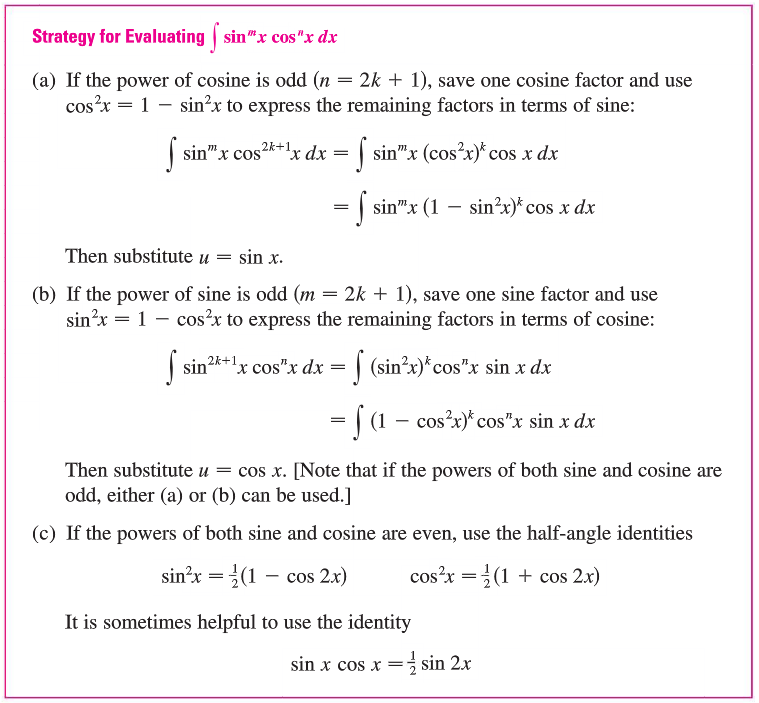
\includegraphics[scale=0.5]{7-2pic1.png}\]

\section*{Tan and Sec}

We can use a similar strategy to evaluate integrals of the form $\ds\int \tan^m x \sec^n x dx$:\\

\begin{itemize}
\item Since $\ds\frac{d}{dx} (\tan x) = \underline{\hspace{1in}}$, we can separate a $\sec^2 x$ factor and convert the remaining (even) power of secant to an expression involving tangent using the identity:\\

\[\underline{\hspace{2.5in}}\]
\item Or, since $\ds\frac{d}{dx} (\sec x) = \underline{\hspace{1.25in}}$, we can separate a $\sec x\tan x$ factor and convert the remaining (even) power of tangent to secant with:\\

\[\underline{\hspace{2.5in}}\]
\end{itemize}

\newpage

\underline{Example 5}: Evaluate $\ds\int \tan^6 x\sec^4 x dx$.\\
\indent

\vspace{4in}

\underline{Example 6}: Find $\ds\int \tan^5 \theta \sec^7 \theta d\theta$.\\
\indent

\vspace{4in}

\[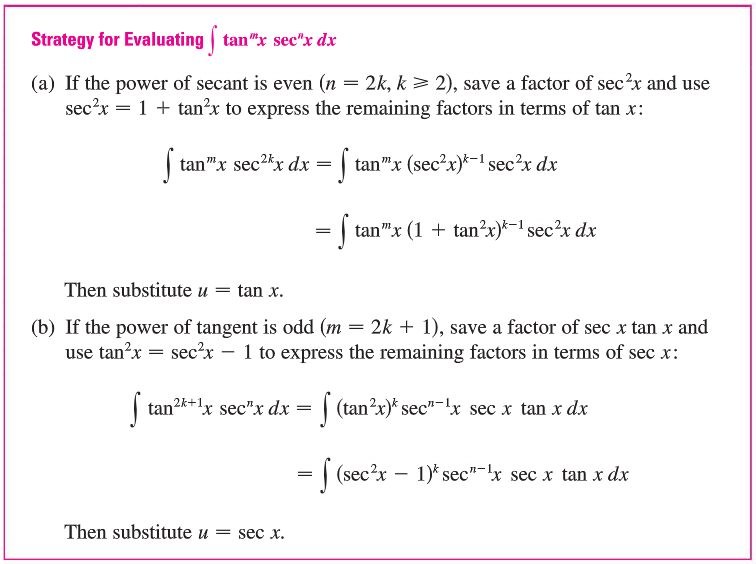
\includegraphics[scale=0.5]{7-2pic2.png}\]
\indent

For other cases, the guidelines are not as clear-cut. We may need to use identities, integration by parts, and occasionally a little ingenuity. We will sometimes need to be able to integrate $\tan x$ or $\sec x$:

\begin{itemize}
\item $\ds\int \tan x dx$\\
\indent\\
\indent\\
\indent\\
\indent\\
\indent\\
\indent\\
\indent\\
\indent\\
\indent\\
\item $\ds\int \sec x dx$\\
\indent\\
\indent\\
\indent\\
\indent\\
\indent\\
\indent\\
\indent\\
\end{itemize}

\indent

\newpage
\underline{Example 7}: Find $\ds\int \tan^3 x dx$.\\
\indent

\vspace{3in}

\underline{Example 8}: Find $\ds\int \sec^3 x dx$.\\
\indent

\vspace{3in}

%\underline{7.2 \#19}: Evaluate $\ds\int \ds\frac{\cos x + \sin 2x}{\sin x}dx$.\\
\indent

\vspace{3.25in}


%----------------------------------------------------------------------------------------

\end{document}